%!TEX program = xelatex
\documentclass[UTF8,fontset=none,11pt,a4paper]{ctexart}
\usepackage{fontspec}
\setmainfont{Avenir Next}
\setsansfont{Avenir Next}
\setCJKmainfont{PingFang SC}
\setCJKsansfont{PingFang SC}
\usepackage[margin=17mm,top=16mm,bottom=16mm]{geometry}
\usepackage{graphicx,xcolor,tabularx,array,multicol,tikz,fancyhdr,hyperref}
\usepackage[most]{tcolorbox}
\usetikzlibrary{arrows.meta,positioning}
\hypersetup{colorlinks=true,urlcolor=[HTML]{1D684F},linkcolor=[HTML]{1D684F}}
\definecolor{ink}{HTML}{1E2B25}
\definecolor{forest}{HTML}{174C3A}
\definecolor{mint}{HTML}{E9F2ED}
\definecolor{slate}{HTML}{5E6C64}
\definecolor{line}{HTML}{D9E2DC}
\definecolor{gold}{HTML}{C79648}
\definecolor{paper}{HTML}{F8F7F2}
\pagecolor{paper}
\color{ink}
\setlength{\parindent}{0pt}
\setlength{\parskip}{0pt}
\renewcommand{\arraystretch}{1.32}
\pagestyle{fancy}
\fancyhf{}
\fancyhead[L]{\footnotesize\color{forest}\bfseries 物资仓库 AI 借还工作台}
\fancyhead[R]{\footnotesize\color{slate}作品介绍 · 演示版本}
\fancyfoot[L]{\footnotesize\color{slate}智创校园 · 浙晓未来}
\fancyfoot[R]{\footnotesize\color{slate}\thepage\ / 7}
\renewcommand{\headrulewidth}{0.4pt}
\renewcommand{\footrulewidth}{0pt}
\setlength{\headheight}{14pt}
\newtcolorbox{softbox}[1][]{enhanced,boxrule=0.5pt,colframe=line,colback=white,
  arc=3mm,left=4mm,right=4mm,top=3mm,bottom=3mm,#1}
\newtcolorbox{greenbox}[1][]{enhanced,boxrule=0pt,colback=mint,
  arc=3mm,left=4mm,right=4mm,top=3mm,bottom=3mm,#1}
\newcommand{\eyebrow}[1]{{\small\bfseries\color{forest}#1}}
\newcommand{\pageheading}[2]{\eyebrow{#1}\par\vspace{2mm}{\fontsize{23}{29}\selectfont\bfseries #2}\par\vspace{3mm}{\color{gold}\rule{24mm}{1.4pt}}\par\vspace{5mm}}
\newcommand{\capsule}[1]{\tikz[baseline=(X.base)]\node[draw=line,fill=white,rounded corners=2mm,
  inner xsep=2.7mm,inner ysep=1.2mm] (X) {\footnotesize\bfseries #1};}
\newcommand{\smalllabel}[1]{{\footnotesize\bfseries\color{forest}#1}}

\begin{document}
\thispagestyle{empty}

% 1 — Cover
\begin{minipage}[c]{0.58\linewidth}
  
\includegraphics[width=15mm]{assets/zju-seal.png}\hspace{3mm}
  \begin{minipage}[c]{0.69\linewidth}
    {\small\bfseries 浙江大学 · 校园场景 AI 应用}\par
    {\footnotesize\color{slate}智创校园 · 浙晓未来｜作品介绍文档}
  \end{minipage}
\end{minipage}\hfill
\begin{minipage}[c]{0.37\linewidth}\raggedleft
  {\footnotesize\color{forest}\bfseries WEB DEMONSTRATION}\par
  {\footnotesize\color{slate}2026 年 10 月 17 日}
\end{minipage}

\vspace{18mm}
\eyebrow{PHOTO · RECOGNIZE · VERIFY}\par\vspace{4mm}
{\fontsize{32}{40}\selectfont\bfseries 物资仓库\par AI 借还工作台}\par\vspace{5mm}
{\Large\color{forest}拍一张照，核对一单物资}\par\vspace{5mm}
{\normalsize\color{slate}借出时把物资集中拍摄，由 AI 识别种类和数量，再与申请清单核对。\par
我们希望用这一步代替逐件人工清点；照片同时留下交接时的现场记录。}

\vspace{9mm}
\smalllabel{核心关键词}\par\vspace{2mm}
\capsule{同框拍照}\hspace{2mm}\capsule{物资识别}\hspace{2mm}\capsule{清单核对}\hspace{2mm}\capsule{库存更新}\hspace{2mm}\capsule{校园借还}

\vspace{12mm}
\begin{softbox}
\begin{minipage}[c]{0.61\linewidth}
  \smalllabel{核心问题}\par\vspace{2mm}
  {\large\bfseries 谁来核对实际借走的物资？}\par\vspace{2mm}
  {\small\color{slate}借出清单靠人填写，管理员还要对着实物逐件清点。物资多、摆放杂时，核对费时，也容易漏看。本作品尝试让 AI 先从同框照片中认出物资并核对数量；看不准的部分再交给管理员。}
\end{minipage}\hfill
\begin{minipage}[c]{0.34\linewidth}
  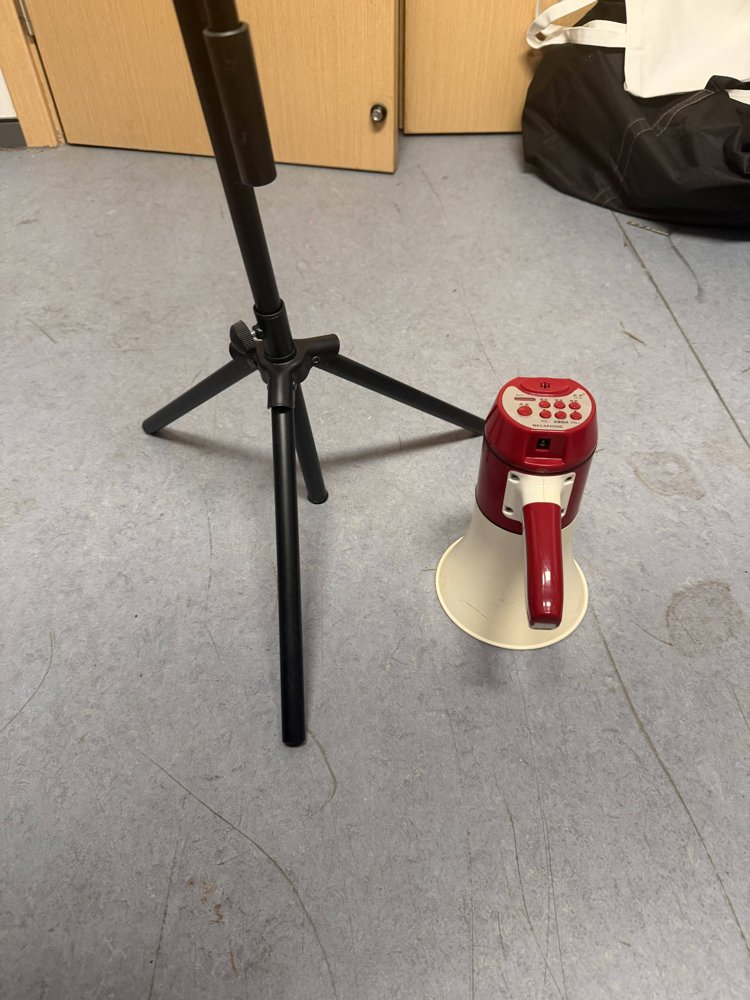
\includegraphics[width=\linewidth,height=50mm,keepaspectratio]{assets/scene.jpg}
\end{minipage}
\end{softbox}

\vfill
\begin{minipage}{0.69\linewidth}
{\small\bfseries 作品形态}\quad 可运行的 Web 演示原型\par\vspace{1mm}
{\small\bfseries 在线体验}\quad\href{https://blog.oppenheimer123.xyz/warehouse-ai/}{blog.oppenheimer123.xyz/warehouse-ai/}
\par\vspace{1mm}
{\small\bfseries GitHub 仓库}\quad\href{https://github.com/Feynman724/warehouse-ai}{github.com/Feynman724/warehouse-ai}
\end{minipage}\hfill
\begin{minipage}{0.28\linewidth}\raggedleft
{\footnotesize\color{slate}作品介绍文档\par V4.0 · 2026.10}
\end{minipage}

\newpage
% 2 — Problem and overview
\pageheading{01 / WHY IT MATTERS}{让照片承担借出核验}
\begin{greenbox}
\smalllabel{作品概要}\par\vspace{2mm}
一次校园活动可能同时借走帐篷、桌椅、喇叭和支架。申请人先填清单，管理员再逐件核对，最后还要更新库存：同一批物资被反复清点和记录。我们设计的方式是把物资放在一个区域拍照，让 AI 识别种类和数量，并与申请清单比对。系统把候选结果交给管理员确认后逐项入账；有差异或看不清时，重点核对异常项目。照片随借还记录保存，归还时也可对照。
\end{greenbox}

\vspace{6mm}
\smalllabel{人工核验卡在哪里}\par\vspace{3mm}
\begin{tabularx}{\linewidth}{@{}>{\bfseries}p{27mm}X X@{}}
\color{forest}现场 & \color{forest}\bfseries 传统方式 & \color{forest}\bfseries 工作台的改进\\\hline
现场清点 & 多种物资混在一起，管理员要逐件辨认、计数。 & 用同框照片识别物资，生成可核对的种类和数量建议。\\
清单比对 & 申请内容与实际拿走的物资可能不一致。 & 把识别结果与申请清单逐项比对，标出多拿、少拿或无法确认的物资。\\
库存维护 & 核对后还要手动改库存，容易漏记。 & 核验通过后逐项入账，保留照片、操作人和库存变动记录。\\
\end{tabularx}

\vspace{8mm}
\smalllabel{从照片到库存的四步}\par\vspace{4mm}
\begin{center}
\begin{tikzpicture}[node distance=2.2mm,every node/.style={font=\small}]
\tikzset{flowbox/.style={draw=line,fill=white,rounded corners=2mm,minimum height=13mm,text width=29mm,align=center}}
\node[flowbox] (a) {\textbf{申请}\par 多物资清单};
\node[flowbox,right=of a] (b) {\textbf{拍照}\par 同框现场};
\node[flowbox,right=of b] (c) {\textbf{识别核验}\par AI 比对清单};
\node[flowbox,right=of c] (d) {\textbf{入账}\par 逐项库存流水};
\draw[-{Stealth[length=2mm]},forest,thick] (a)--(b);
\draw[-{Stealth[length=2mm]},forest,thick] (b)--(c);
\draw[-{Stealth[length=2mm]},forest,thick] (c)--(d);
\end{tikzpicture}
\end{center}

\vspace{4mm}
\begin{softbox}
\smalllabel{核验规则}\par\vspace{2mm}
\textbf{当前演示版的模型结果不直接改变库存。} 管理员对照照片和申请清单确认实际件数后，系统一次写入整单库存流水。模型没有覆盖某类物资、数量不确定或照片看不清时，界面保留待核对状态；照片也不替代对缺损状况的判断。
\end{softbox}

\vspace{3mm}
\smalllabel{仓库真实物资}\par\vspace{1mm}
\begin{minipage}[c]{0.31\linewidth}\centering
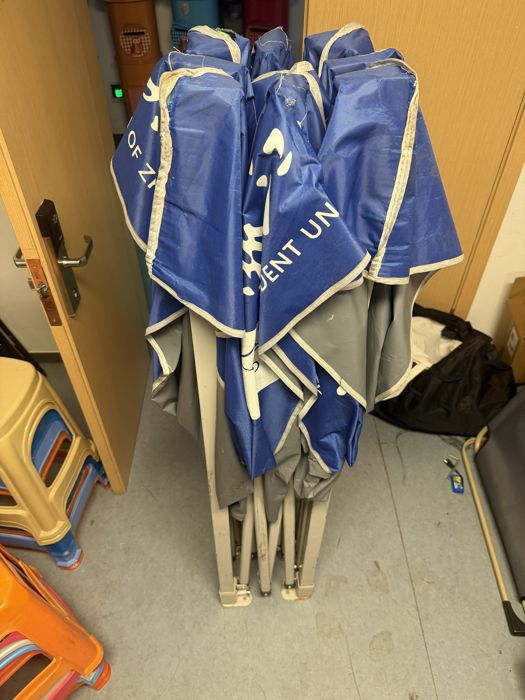
\includegraphics[width=\linewidth,height=20mm,keepaspectratio]{assets/tent.jpg}\par{\footnotesize 帐篷}
\end{minipage}\hfill
\begin{minipage}[c]{0.31\linewidth}\centering
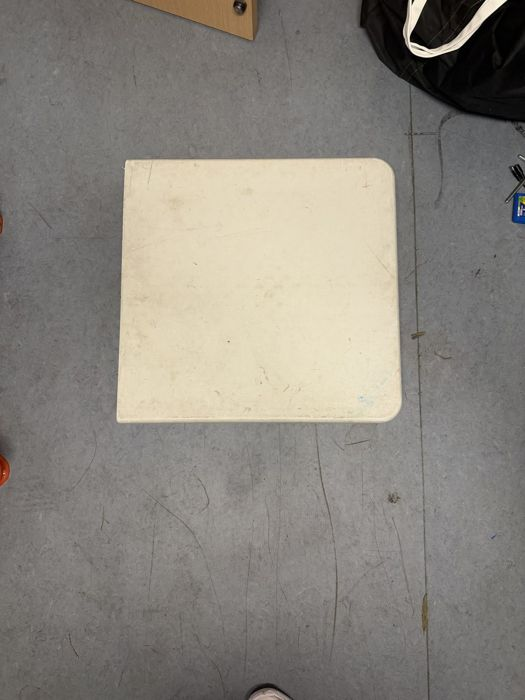
\includegraphics[width=\linewidth,height=20mm,keepaspectratio]{assets/table.jpg}\par{\footnotesize 折叠桌}
\end{minipage}\hfill
\begin{minipage}[c]{0.31\linewidth}\centering
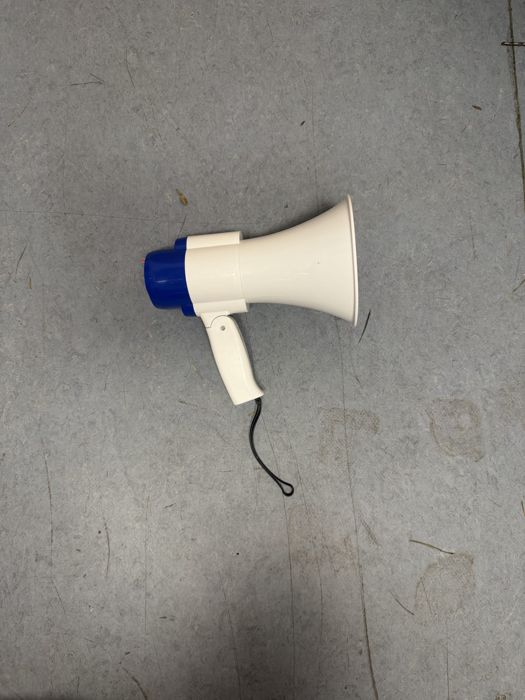
\includegraphics[width=\linewidth,height=20mm,keepaspectratio]{assets/megaphone.jpg}\par{\footnotesize 喇叭}
\end{minipage}

\newpage
% 3 — Product and evidence
\pageheading{02 / HOW IT WORKS}{先识别，再核对，再入账}
\begin{minipage}[t]{0.42\linewidth}
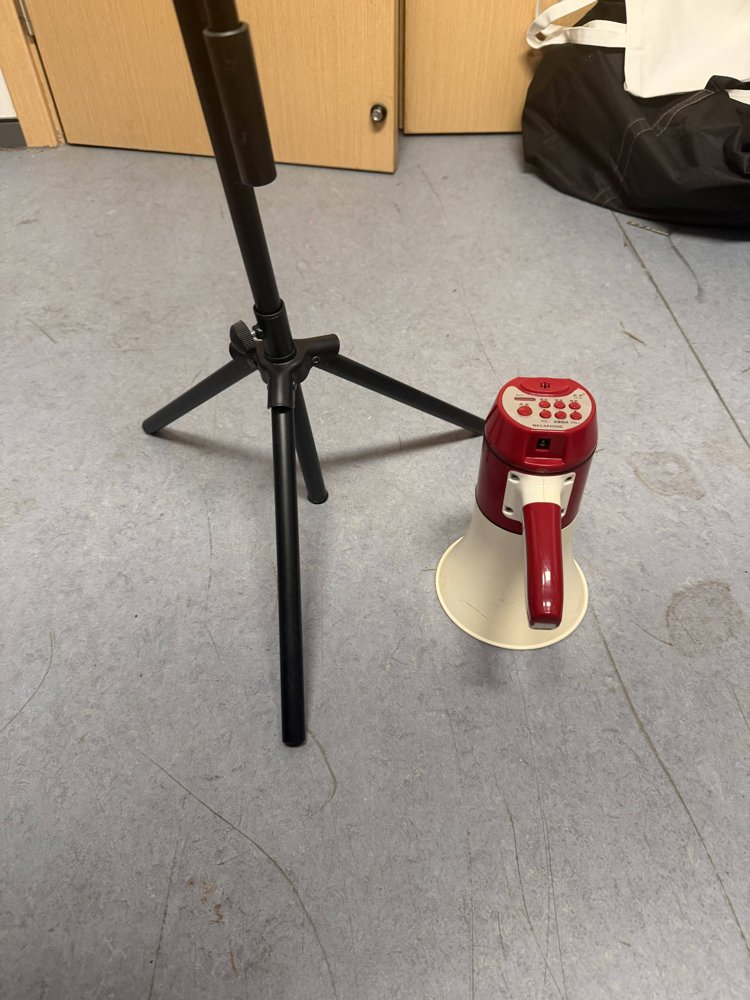
\includegraphics[width=\linewidth,height=112mm,keepaspectratio]{assets/scene.jpg}\par\vspace{2mm}
{\footnotesize\color{slate}实拍样例：喇叭与麦架放置在同一画面。}
\end{minipage}\hfill
\begin{minipage}[t]{0.54\linewidth}
\begin{softbox}
\smalllabel{01｜申请与审批}\par\vspace{1.5mm}
师生一次选择多类物资及数量；管理员批准或填写拒绝理由，改判记录可追溯。
\end{softbox}\vspace{3mm}
\begin{softbox}
\smalllabel{02｜拍摄与清单比对}\par\vspace{1.5mm}
把本次物资集中摆放、拍摄一张现场照。AI 给出物资种类、数量建议，系统逐项对照申请清单，并标出无法确认的项目。
\end{softbox}\vspace{3mm}
\begin{softbox}
\smalllabel{03｜库存与归还}\par\vspace{1.5mm}
管理员确认实际借出件数后，系统逐项扣减库存并记录流水。归还再次拍照，管理员核对完好与缺损数量后更新库存。
\end{softbox}
\end{minipage}

\vspace{7mm}
\begin{greenbox}
\smalllabel{当前可现场展示的效果}\par\vspace{2mm}
\textbf{已实现：}多物资申请、审批、同框拍照、模型识别、清单比对、管理员复核、库存更新和记录回看。网页可打开摄像头，连续发送当前画面，由服务器上的模型返回实时候选框。\par\vspace{1.2mm}
\textbf{现场演示：}把“喇叭 + 麦架”放进画面，展示模型实时给出的两个候选框；也可上传实拍照片走同一推理流程。候选结果不直接修改库存，正式借还仍由管理员确认。
\end{greenbox}

\newpage
% 4 — Context, outcomes and honest status
\pageheading{03 / APPLICATION}{从学生组织物资室出发}
\begin{minipage}[t]{0.48\linewidth}
\smalllabel{落地应用场景}\par\vspace{3mm}
\begin{softbox}
\textbf{学生会与院系团委物资室}\par\vspace{1mm}
帐篷、桌椅、指示牌、喇叭等跨类别物资的集中借还，是本原型最直接的应用场景。
\end{softbox}\vspace{3mm}
\begin{softbox}
\textbf{校园活动交接}\par\vspace{1mm}
活动前后的多批次领用和归还，可用照片、申请清单和库存流水形成统一的交接记录。
\end{softbox}\vspace{3mm}
\begin{softbox}
\textbf{社团与公共器材室}\par\vspace{1mm}
对高频借用、易损或成套器材，保留每次借还的现场影像和责任链。
\end{softbox}
\end{minipage}\hfill
\begin{minipage}[t]{0.48\linewidth}
\smalllabel{预期应用成效}\par\vspace{3mm}
\begin{greenbox}
\textbf{减少逐件清点}\par\vspace{1mm}
识别可靠时，管理员核对系统给出的物资清单，不必从头逐件辨认和计数。
\end{greenbox}\vspace{3mm}
\begin{greenbox}
\textbf{减少清单与实物出入}\par\vspace{1mm}
借出前提示识别结果与申请清单的差异，把问题留在交接现场处理。
\end{greenbox}\vspace{3mm}
\begin{greenbox}
\textbf{库存有据可查}\par\vspace{1mm}
核验后逐项入账，借还照片与变动记录一起保存；不确定时仍由管理员确认。
\end{greenbox}
\end{minipage}

\vspace{7mm}
\smalllabel{已验证的原型边界}\par\vspace{3mm}
\begin{softbox}
当前组合开放词表模型、红色喇叭视觉提示和用仓库照片微调的检测模型。提供的\textbf{8 张混放照片}已全部用于最终演示模型训练；照片中标出的 29 个目标里，系统给出 28 个同类候选框（IoU≥0.3），仍漏掉 1 个手电筒。当前没有独立测试集，训练照片上的结果不能代表新场景准确率，也不足以支持自动扣库。归还影像的整体差异只能提示复核，\textbf{不能自动判定损坏}。下一步需要补拍并标注不同场景的混放照片，留出独立测试集检验类别、计数和误扣情况；达到要求前，实际借还仍由管理员复核。
\end{softbox}

\vspace{6mm}
\begin{minipage}[c]{0.72\linewidth}
\smalllabel{在线演示}\par\vspace{1mm}
\href{https://blog.oppenheimer123.xyz/warehouse-ai/}{https://blog.oppenheimer123.xyz/warehouse-ai/}\par\vspace{2mm}
{\footnotesize\color{slate}演示版已部署；真实库存与沙盒演示数据分离。}
\end{minipage}\hfill
\begin{minipage}[c]{0.25\linewidth}\raggedleft
{\footnotesize\color{forest}\bfseries 让每一次借还\par 都有据可查。}
\end{minipage}

\newpage
% 5 — Data and training
\pageheading{04 / DATA \& TRAINING}{从仓库实拍到专用检测器}
\begin{greenbox}
\smalllabel{为什么要训练自己的模型}\par\vspace{2mm}
通用检测器认识“椅子”，未必认识仓库里的“麦架”“指示牌”，更难在一张拥挤的交接照里数清各类物资。我们将真实仓库照片整理成\textbf{10 类目标检测数据}，以预训练 YOLO11n 为起点微调，使模型学习本仓库物资的外形、尺度和混放背景。
\end{greenbox}

\vspace{5mm}
\smalllabel{数据如何进入训练}\par\vspace{2mm}
\begin{tabularx}{\linewidth}{@{}>{\bfseries}p{28mm}X@{}}
\color{forest}原始素材 & 23 张单品照、8 张混放照，均为提供的仓库实拍；最终模型使用全部 31 张。\\
\color{forest}清洗与标注 & 去除照片 EXIF、缩小图像；按“喇叭、帐篷、手电筒、扫帚、折叠桌、指示牌、椅子、水桶、画架、麦架”统一类别，为物体画边界框，保存为 YOLO 格式。混放照共标注 29 个目标；遮挡或小物体的框有近似误差。\\
\color{forest}训练输入 & 将类别、框坐标与图像绑定；模型以 640×640 输入学习位置与类别，利用 Mosaic 拼接、左右翻转和尺度扰动增加摆放变化。\\
\end{tabularx}

\vspace{5mm}
\smalllabel{三段式训练：从辨认单品到处理同框照片}\par\vspace{2mm}
\begin{softbox}
\begin{tabularx}{\linewidth}{@{}>{\bfseries}p{24mm}p{36mm}X@{}}
\color{forest}阶段 & \color{forest}\bfseries 数据与设置 & \color{forest}\bfseries 解决的问题\\\hline
1. 单品起步 & 23 张单品照；70 轮，Mosaic 0.7。 & 先让模型学会 10 类物资的基本轮廓。\\
2. 混放适配 & 单品照＋首批 4 张混放照；21 轮后提前停止。 & 学习遮挡、远近和同框背景；从上一阶段权重继续训练。\\
3. 演示定型 & 全部 31 张；80 轮，Mosaic 0.25。 & 纳入后续 4 张混放照，降低过强的拼接增强，让最终模型贴近真实拍摄构图。\\
\end{tabularx}
\end{softbox}

\vspace{4mm}
\begin{minipage}[t]{0.48\linewidth}
\smalllabel{训练配置}\par\vspace{1mm}
{\small 图像边长 640、批量 8；在 Apple M4 的 MPS 上训练。最终权重导出为 ONNX（opset 17），服务器用 ONNX Runtime 在 CPU 上推理。}
\end{minipage}\hfill
\begin{minipage}[t]{0.48\linewidth}
\smalllabel{关键取舍}\par\vspace{1mm}
{\small 物资类别固定，所以采用有监督专用模型；同时保留开放词表分支补充识别。训练照片数量少，专用模型的好结果不能当成跨场景泛化证明。}
\end{minipage}

\newpage
% 6 — Inference details
\pageheading{05 / INFERENCE ENGINE}{三路视觉结果，合成一张清单}
\begin{softbox}
\smalllabel{一帧照片的推理链路}\par\vspace{2mm}
{\small 1. 浏览器采集 JPEG $\rightarrow$ 2. 服务端纠正方向、检查画质 $\rightarrow$ 3. 等比缩放到 640×640 $\rightarrow$ 4. 三路目标检测 $\rightarrow$ 5. 去重、计数并比对清单。}
\end{softbox}

\vspace{5mm}
\begin{tabularx}{\linewidth}{@{}>{\bfseries}p{35mm}X@{}}
\color{forest}识别分支 & \color{forest}\bfseries 职责\\\hline
YOLOE-26s · 文字提示 & 输入“folding table”“camping tent”等 12 个英文提示词，再映射到 10 个仓库类别，为形态较通用的物资提供开放词表候选。\\
YOLOE-26s · 视觉提示 & 用实拍红色喇叭作为参考，让模型在新画面中寻找同类目标；针对仅靠文字提示容易漏掉的具体外观补一条通路。\\
YOLO11n · 仓库专用 & 使用本仓库带框照片微调，优先处理麦架、指示牌等场景相关的类别；权重以约 10 MB 的 ONNX 文件部署。\\
\end{tabularx}

\vspace{5mm}
\smalllabel{后处理并非简单相加}\par\vspace{2mm}
\begin{greenbox}
三路输出先按各自置信度门槛筛选；对易误认的椅子、扫帚及专用模型的不同类别设置更严格阈值。每路以 IoU $>0.50$ 抑制重叠框，合并时对\textbf{同类别且 IoU $>0.35$} 的候选再去重。边界框还原到原图坐标后，同类剩余框的个数才作为“建议数量”。这些阈值是针对现有演示照片调出的工程参数，尚未在独立测试集上校准。
\end{greenbox}

\vspace{5mm}
\smalllabel{真实模型输出示例}\par\vspace{2mm}
\begin{minipage}[t]{0.48\linewidth}\centering
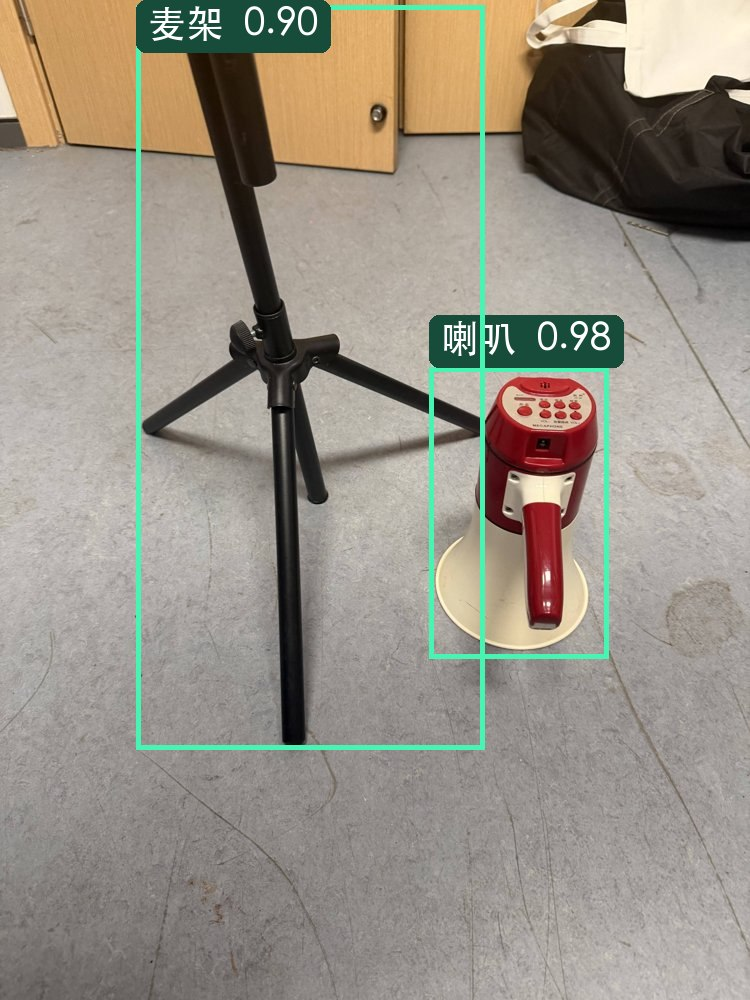
\includegraphics[width=\linewidth,height=67mm,keepaspectratio]{assets/recognition-demo.jpg}\par\vspace{1mm}
{\footnotesize\color{slate}喇叭＋麦架的现场照片}
\end{minipage}\hfill
\begin{minipage}[t]{0.48\linewidth}\centering
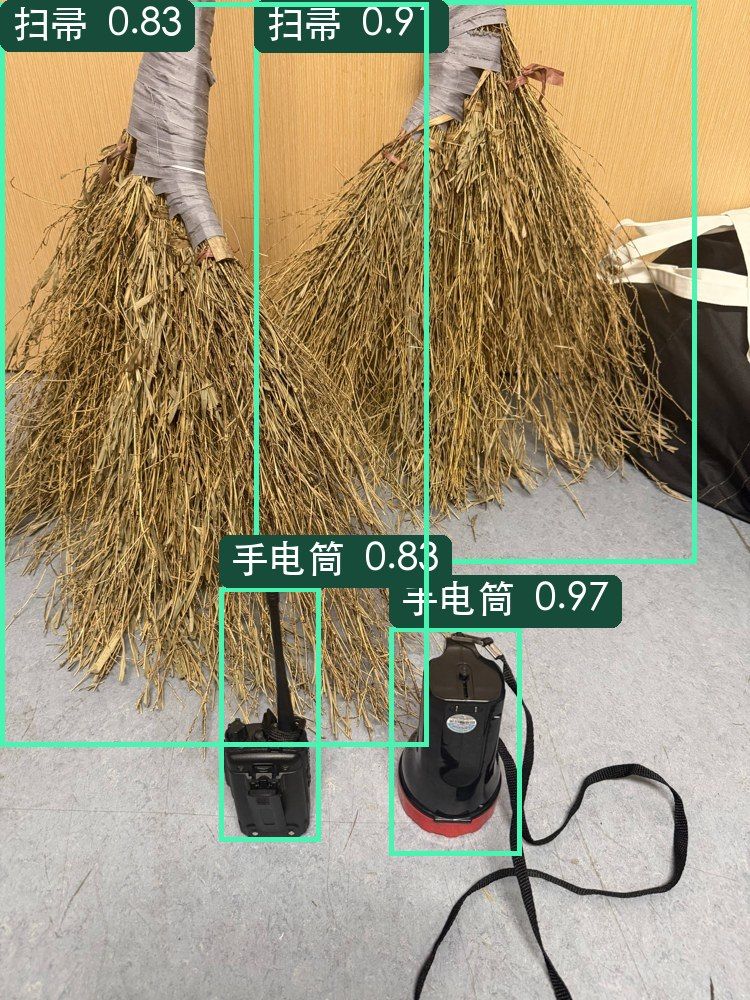
\includegraphics[width=\linewidth,height=67mm,keepaspectratio]{assets/recognition-mixed.jpg}\par\vspace{1mm}
{\footnotesize\color{slate}混放训练照片中的候选框}
\end{minipage}

\vspace{2mm}
{\footnotesize\color{slate}图中框与分数由当前模型实际推理结果绘制；第二张照片已参与训练，不能作为独立测试证据。}

\newpage
% 7 — System and evaluation
\pageheading{06 / SYSTEM \& EVIDENCE}{让识别结果可用，也可追溯}
\smalllabel{前后端如何协同}\par\vspace{2mm}
\begin{softbox}
{\small 手机网页通过摄像头读取当前画面，最长边压至 640 像素，以约 1.5 秒间隔逐帧提交；服务器缓存三个 ONNX 推理会话并串行处理实时请求。返回每个候选的类别、置信度与归一化位置，前端把框画回原图，显示按类别汇总的件数。单张照片上传与实时画面走同一识别流程。}
\end{softbox}

\vspace{5mm}
\smalllabel{为什么有模型，还要保留管理员确认}\par\vspace{2mm}
\begin{greenbox}
真实借还不是只看“有没有框”。用户先提交一单多物资申请，审批后拍摄同框照片；系统保存原始证据、识别建议和申请清单，并指出数量差异。\textbf{管理员逐项确认实际借出件数，数据库事务才更新库存与流水。} 归还时再次留照，管理员分别填完好与缺损件数。当前三路模型启用时，自动入账资格被明确关闭；画面预览更不会改库存。这样即使漏检、误认，也不会让模型直接误扣库存。
\end{greenbox}

\vspace{5mm}
\smalllabel{能复核的结果与不能越过的边界}\par\vspace{2mm}
\begin{tabularx}{\linewidth}{@{}>{\bfseries}p{31mm}X@{}}
\color{forest}训练照复查 & 8 张混放照片共 29 个手工标注目标；组合模型找到 28 个同类候选框，匹配条件为 IoU $\geq 0.30$，漏掉 1 个手电筒。\\
\color{forest}评估性质 & 这 8 张都参与了最终训练，因此 28/29 是\textbf{训练照片回查}，不是独立测试准确率；它也没有统计误检、计数全对率或跨场景稳定性。\\
\color{forest}下一步验收 & 在不同房间、光照、角度、遮挡和数量组合中补拍照片；按拍摄场景划分训练与未参与调参的测试集，报告逐类召回、误检、数量误差和库存误扣风险。\\
\end{tabularx}

\vspace{5mm}
\begin{softbox}
\smalllabel{演示部署与资料}\par\vspace{2mm}
{\small 在线服务：\href{https://blog.oppenheimer123.xyz/warehouse-ai/}{blog.oppenheimer123.xyz/warehouse-ai/}。GitHub：\href{https://github.com/Feynman724/warehouse-ai}{github.com/Feynman724/warehouse-ai}（目前为私有仓库，需授权访问）。仓库包含标注、可重跑的训练照片检查脚本和推理流程；演示强调\textbf{真实模型、真实照片、真实库存事务}，并区分训练照效果与无人值守扣库所需的验证结论。}
\end{softbox}

\end{document}
